\chapter{Constant Trajectories}
\section{Introduction}
In our investigation of solutions to $Ax = 0$, where $x$ is non-zero but some $x_i = 0$, we focus on cases where $n > 2$, excluding the trivial scenario of $n = 1$ where $A$ reduces to the zero matrix. Assuming the irreducibility of $A$ and the absence of cycles longer than 2 in $SD(A)$, if $Ax = 0$ and $x \neq 0$, we can divide the signed digraph $SD(A)$ and the graph $G(A)$ into distinct subgraphs.

To achieve this partitioning, we introduce the concept of a white block, which represents a maximal connected subgraph of nodes in $SD(A)$ corresponding to non-zero components of $x$. Nodes not included in white blocks are labeled as black and form part of black blocks.

This partitioning scheme can be understood through what we term as a "color test".

\section{Constant Trajectories and 0-coloring}
\begin{dfn}
	A constant trajectory $x(t) \in \mathbb{R}^n$ for $\dot{x}_i = \sum_{j=1}^n a_{ij}x_j$ satisfies $\dot{x}_i = 0$ and $x_i \neq 0$ for some $i$.
\end{dfn}
\begin{dfn}
	 A 0-coloring is a scheme for coloring all nodes of $SD(A)$ which has no $k$-cycle, $k > 2$, black or white, so that:
	\begin{enumerate}
		\item no black node is a neighbor of exactly one white node;
		\item each maximal white block as a subgraph is either: a single undistinguished node; or a digraph which has at least two nodes, which has each end node distinguished, and which is not $\lambda$-consistent.
	\end{enumerate}
\end{dfn}

\begin{example}
Consider the matrix 
\begin{center}

$\tilde{A}=
\begin{bmatrix}
	3 & 0 & -3 & 0 & 0 \\
	0 & 1 & -2 & 2 & 0 \\
	-2 & 1 & 2 & 0 & 0 \\
	0 & 3 & 0 & 0 & 0 \\
	0 & 0 & 0 & 0 & 0 \\
\end{bmatrix}$
and let 
$x=
\begin{bmatrix}
	1 \\
	0 \\
	1 \\
	1 \\
	0 \\
\end{bmatrix}$
\end{center}
be a solution corresponding to the equation $Ax=0$. Thus, we color nodes $\{1,3,4\}$ white since the corresponding $x_i$ values for nodes $\{1,3,4\}$ are non-zero. Conversely, nodes $\{2,5\}$ are colored black, indicating that the corresponding $x_i$ values for these nodes are zero. Additionally, this coloring satisfies the criteria of 0-coloring, as node 2 is a neighbor of two white nodes, i.e., nodes 3 and 4.
\begin{center}
	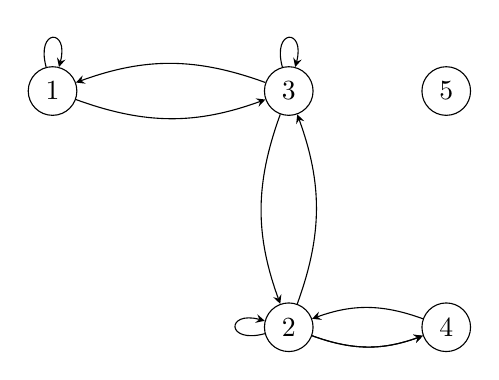
\begin{tikzpicture}[>=stealth]
		% Nodes in a circle
		\node[circle, draw] (1) at (0,0) {1};
		\node[circle, draw] (2) at (3,-3) {2};
		\node[circle, draw] (3) at (3,0) {3};
		\node[circle, draw] (4) at (5,-3) {4};
		\node[circle, draw] (5) at (5,0) {5};
		
		% Edges
		\draw[->] (1) to[bend right=20] (3);
		\draw[->] (2) to[bend right=20] (4);
		\draw[->] (1) to[loop above] (1);
		\draw[->] (3) to[loop above] (3);
		\draw[->] (2) to[loop left] (2);
		
		\draw[->] (2) to[bend right=20] (3);
		\draw[->] (3) to[bend right=20] (2);
		
		\draw[->] (3) to[bend right=20] (1);
		\draw[->] (2) to[bend right=20] (4);
		
		\draw[->] (4) to[bend right=20] (2);
		
	\end{tikzpicture}
\end{center}

\end{example}
\begin{thm}
	Suppose $A$ is an irreducible matrix of order $\geq 2$ and $SD(A)$ contains no $k$-cycle, $k > 2$. Then there exists $\tilde{A} \in Q(A)$ and a vector $x \neq 0$ satisfying $\tilde{A}x = 0$ if and only if $SD(A)$ admits a 0-coloring with at least one white node.
\end{thm}

\begin{proof}
	 First, we are going to prove in a forward direction i.e, $SD(A)$ admits a 0-coloring with at least one white node.
	 Suppose, $n \geq 2$, and we have a non-zero solution $x$ to the equation $Ax = 0$, with the constraint $x \neq 0$. We proceed by coloring all nodes corresponding to non-zero entries in $x$ as white, while the remaining nodes are colored black.
	
   	When all $x_i \neq 0$, Theorem 1 implies condition (ii) is satisfied, as all nodes are white. However, in case where both black and white nodes exist, we need to ensure condition (i) holds true. This condition becomes evident when we examine the equation corresponding to the $j$th row in $Ax = 0$ for some $x_j = 0$. we see condition (i) must be fulfilled.
	
	Each white block represents a subsystem of equations $\bar{A}\bar{x}=0$ within $Ax = 0$, adhering to the conditions outlined in Theorem 1. Consequently, every white block must fulfill condition (ii) to maintain consistency with the theorem's requirements.
	
	Now, let's consider the \textbf{converse} scenario: assume $SD(A)$ admits a 0-coloring with at least one white node. Here's how we construct a non-zero vector $x$ that satisfies $\tilde{A}x = 0$.
	
	We begin by examining the subsystem of equations $\tilde{A}x = 0$ associated with a white block. According to Theorem 1, such a subsystem has a solution where each component is non-zero. We define the components of the complete vector $x$ accordingly.
	
	Suppose node $j$ is black and connected to a node within this white block. By condition (i), node $j$ must be linked to other white nodes $k_1, k_2, \ldots, k_q$, where $q \geq 1$. We assign arbitrary positive values to $|\tilde{a}_{jk_{i}}|$ and choose non-zero ${x_{k_i}}$ values that satisfy the $j$th row equation in $\tilde{A}x = 0$. Using the idea of Theorem 2.1.2, we extend these $x$-values throughout their respective white blocks. Given that $G(A)$ forms a tree, we can systematically extend these values to all white nodes and black nodes connected to white nodes.
	
	We assign arbitrary magnitudes to all other entries in $\tilde{A}$ corresponding to edges in $SD(A)$ originating from black nodes, while setting the components of $x$ corresponding to black nodes to zero. This process completes the construction of $\tilde{A}$ and $x$ satisfying $\tilde{A}x = 0$ with $x \neq 0$.

\end{proof}
\begin{example}
	Let's consider the scenario where $SD(A)$ allows a 0-coloring with at least one white node. We aim to find a non-zero solution $x$ satisfying $Ax = 0$. We begin by examining the subsystem of equations $Ax = 0$ associated with a white block, comprising nodes $\{1,3\}$, assuming they form the maximal white block. Additionally, nodes 4 and 6 are also white but are undistinguished nodes. According to Theorem 2.1.2, such a subsystem has a non-zero solution for each component. Let nodes $\{2,5\}$ be black, and node 2 is linked to white nodes $\{1,3,4,6\}$.
	
	We construct the matrix $\tilde{A}$ as follows:
	\begin{center}
		$\tilde{A}=$
		$\begin{bmatrix}
			3 & 0 & -3 & 0 & 0 & 0\\
			0 & \tilde{a}_{22} & \tilde{a}_{23} & \tilde{a}_{24} & 0 & \tilde{a}_{26}\\
			-2 & \tilde{a}_{32} & 2 & 0 & 0 & 0\\
			0 & \tilde{a}_{42} & 0 & 0 & 0 & 0\\
			0 & 0 & 0 & 0 & 0 & 0\\
			0 & \tilde{a}_{62} & 0 & 0 & 0 & 0\\
		\end{bmatrix}$
	\end{center}
	And let $x$ be:
	\begin{center}
		$x=$
		$\begin{bmatrix}
			1 \\
			0 \\
			1 \\
			x_4 \\
			0 \\
			x_6
		\end{bmatrix}$
	\end{center}
	
	Node 4 is connected to other white nodes 4 and 6. We choose arbitrary positive values for $|\tilde{a}_{24}|$ and $|\tilde{a}_{24}|$ and determine $x_4$ and $x_6$ so that they satisfy the 2nd row equation in $\tilde{A}x=0$. We assign arbitrary magnitudes to all other entries in $\tilde{A}$ corresponding to edges originating from black nodes, while setting the components of $x$ corresponding to black nodes to zero. This process completes the construction of $\tilde{A}$ and $x$, ensuring $\tilde{A}x = 0$ with $x \not\equiv 0$. Hence, $\tilde{A}$ and $x$ using the algorithm of the proof are given by:
	\begin{center}
		$\tilde{A}=$
		$\begin{bmatrix}
			3 & 0 & -3 & 0 & 0 & 0\\
			0 & 1 & 4 & -2 & 0 & 1\\
			-2 & 1 & 2 & 0 & 0 & 0\\
			0 & 3 & 0 & 0 & 0 & 0\\
			0 & 0 & 0 & 0 & 0 & 0\\
			0 & -1 & 0 & 0 & 0 & 0\\
		\end{bmatrix}$
and
		$x=$
		$\begin{bmatrix}
			1 \\
			0 \\
			1 \\
			1 \\
			0 \\
			-2
		\end{bmatrix}$
	\end{center}
Its associated signed digraph is given by;
\begin{center}
	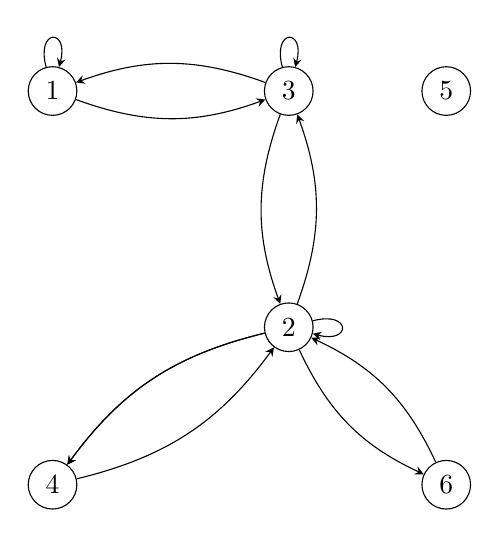
\begin{tikzpicture}[>=stealth]
		% Nodes in a circle
		\node[circle, draw] (1) at (0,0) {1};
		\node[circle, draw] (2) at (3,-3) {2};
		\node[circle, draw] (3) at (3,0) {3};
		\node[circle, draw] (4) at (0,-5) {4};
		\node[circle, draw] (5) at (5,0) {5};
		\node[circle, draw] (6) at (5,-5) {6};
		
		% Edges
		\draw[->] (1) to[bend right=20] (3);
		\draw[->] (2) to[bend right=20] (4);
		\draw[->] (1) to[loop above] (1);
		\draw[->] (3) to[loop above] (3);
		\draw[->] (2) to[loop right] (2);
		
		\draw[->] (2) to[bend right=20] (3);
		\draw[->] (3) to[bend right=20] (2);
		
		\draw[->] (3) to[bend right=20] (1);
		\draw[->] (2) to[bend right=20] (4);
		
		\draw[->] (4) to[bend right=20] (2);
		%\draw[->] (5) to[bend right=20] (4);
		
		\draw[->] (2) to[bend right=20] (6);
		\draw[->] (6) to[bend right=20] (2);
		
	\end{tikzpicture}
\end{center}
\end{example}

\subsection*{Undirected Block graph B(A)}
To explore the presence of multiple eigenvalues in matrix $A$, we introduce the concept of an undirected block graph denoted as $B(A)$. We begin by assuming the existence of a nontrivial 0-coloring scheme for $SD(A)$. In this scheme, we remove from $SD(A)$ all black nodes that are not connected to any white nodes, along with any edges connected to or from these isolated black nodes.

The nodes of $B(A)$ are then composed of the remaining black nodes denoted as ${b_1, b_2, \ldots}$, along with the maximal white blocks denoted as ${w_1, w_2, \ldots}$. An edge ${(b_i, w_j)}$ belongs to $B(A)$ if and only if some node in $b_i$ is connected by a 2-cycle to some node in $w_j$.
Now, we define the concept of branching within $B(A)$. 
\begin{dfn}
	$B(A)$ is branched at a black node if that black node in $B(A)$ is connected to more than two white nodes
\end{dfn} 

\begin{thm}
	Suppose $A$ is irreducible and $SD(A)$ contains no $k$-cycle, $k > 2$. Then 0 is an eigenvalue in at least two Jordan blocks of some $\tilde{A} \in Q(A)$ if and only if $SD(A)$ admits a 0-coloring for which $B(A)$ is branched at a black node.
\end{thm}

\begin{proof}
	Suppose we have a matrix $\tilde{A}$ belonging to the set $Q(A)$, and 0 appears as an eigenvalue in two or more Jordan blocks of $A$. In such a case, there must exist two linearly independent solutions $x$ and $y$ to the equations $\tilde{A}x = \tilde{A}y = 0$.This is because the Jordan Canonical Form (JCF) of a matrix $\tilde{A}$ is a block-diagonal matrix consisting of Jordan blocks, where each Jordan block corresponds to an eigenvalue of $A$. If 0 is an eigenvalue with more than one Jordan block, it implies that there are multiple linearly independent eigenvectors associated with the eigenvalue 0, each corresponding to a different Jordan block.
	 
	We select $x$ in such a way that the number of components with $x_i = 0$ is maximal. If the 0-colorings associated with $x$ and $y$ are identical, then it follows that $x_i = 0$ if and only if $y_i = 0$. By rearranging and renumbering the components, we can arrange for $x_i$ and $y_i$ to be equal and non-zero. Consequently, the 0-coloring associated with $x - y$ would have more zero components than $x$, leading to a contradiction. Therefore, we can assume, without loss of generality, that the 0-coloring associated with $x$ contains the minimal number of white nodes, and that the 0-colorings associated with $x$ and $y$ are distinct.
	
	Consider a scenario where we have a white block in the 0-coloring for vector $x$, denoted as $\bar{x}$, with associated submatrix $\bar{A}$. Let's suppose that this white block is attached at node $i$ to exactly one black node, denoted as node $j$. Such a configuration must always exist. 
	
	Now, let's introduce another vector $y$ with its corresponding 0-coloring. If node $j$ is white in the 0-coloring for $y$, then we can express $\bar{A}\bar{y} + \xi = 0$, where $\xi$ is a vector with only one non-zero entry corresponding to the attachment of node $i$ to the white node $j$. 
	
	Since any vector in the kernel of $\bar{A}$ must be proportional to $\bar{x}$, we can infer that $\bar{y_k} = \alpha \bar{x_k}$ for all nodes in the white block, including node $i$. Upon considering the $i$th row equation, we find $\xi_i = 0$, leading to a contradiction. This contradiction indicates that node $j$ must be black in the 0-coloring for $y$.
	
	By leveraging the tree structure of $G(A)$, this reasoning extends to all nodes that are black in the 0-coloring for $x$ and are attached to white nodes. It demonstrates that no white block of the 0-coloring for $y$ can entirely contain a white block of the 0-coloring for $x$. 
	
	Consequently, if the two colorings differ, it implies that some white block and its adjacent black nodes from the coloring for $x$ lie completely within a black block of the coloring for $y$. 
	
	By coloring a node of $SD(A)$ white if it's white in either the $x$ or the $y$ 0-coloring, and black otherwise, we effectively create a 0-coloring for $SD(A)$. The associated block graph $B(A)$ resulting from this coloring is branched.


	\textbf{For the converse part}, let's consider a 0-coloring for $SD(A)$ exists, and the associated block graph $B(A)$ is branched. Using the reasoning from the first part of Theorem 3, we can construct a vector $y$ and a modified matrix $\tilde{A}$ such that $\tilde{A}y = 0$, ensuring that $y_i \neq 0$ if and only if node $i$ is white in the 0-coloring.
	
	This implies that the components of $y$ corresponding to black nodes are zero, while the edge values from black nodes can take arbitrary values. Within a branched component of $B(A)$, there exists a straight path with white block end nodes. By recoloring all nodes of $SD(A)$ not in this straight path to black, we achieve a distinct 0-coloring.
	
	Using Theorem 4.2.3 once more, we can construct a new vector $x$ (with the same modified matrix $\tilde{A}$) that is not proportional to $y$, but still satisfies $\tilde{A}x = 0$. This process demonstrates how, starting from a branched block graph $B(A)$, we can iteratively generate distinct solutions to the system of equations $\tilde{A}x = 0$ with unique 0-colorings.

\end{proof}